\section{Experiments}
\label{sec:experiment}

\subsection{Learning methods}

Here, we take the first attempt to quantify computationally the
synthesizability of images. For this purpose, we build (1) a
classifier to distinguish between synthesizable texture examples, and
unsynthesizable ones, (2) a regression model that can predict the
synthesizability of a given image, and (3) an additional classifier to
suggest the `best' ETS method to synthesize the given example.  All
approaches are learned on the $2000$ general textures, with the set of
features described above.  In implementation, linear SVMs and logist
regression were employed for the learning. The parameter $C$ was
obtained by a $5$-fold cross-validation.

\subsection{Effectiveness of features}
In this section, we validate the effectiveness of Homogeneity,
Repetitiveness, and Regularity as general texture analysis
features. The evaluation was performed on $600$ randomly chosen image
pairs from the $2000$ general textures. For each property, each pair
is manually labeled to $1$ or $0$, indicating the first image owns the
property more or less than the second one.  We compared the results
detected by our method to the annotations and reported the accuracy in
Table~\ref{table:fet}. From the table, it is obvious that the
automatic methods we designed for the three texture features performs
fairly well. The features can be used for other texture analysis tasks
rather than just image synthesizability.

\begin{table}[tb] \footnotesize 
$\begin{array}{ccccc}
\begin{tabular}{|c||c||}
\hline 
\multicolumn{1}{|c||}{Methods} \\ \hline \hline
Accuracy \\  \hline
\end{tabular}

\begin{tabular}{|c|c|}
\hline
\multicolumn{1}{|c|}{Homogeneity} \\ \hline \hline
79.4\%  \\ \hline
\end{tabular}

\begin{tabular}{|c|c|}
\hline
\multicolumn{1}{|c|}{Repetitiveness} \\ \hline \hline
82.5\%  \\ \hline
\end{tabular}

\begin{tabular}{|c|c|}
\hline 
\multicolumn{1}{|c|}{Regularity} \\ \hline \hline
75.2\%  \\  \hline
\end{tabular}
\end{array} $
\vspace{1mm}
\centering 
\caption{ Accuracy of the estimation of three texture properties. 
} \label{table:fet}
\end{table}

\subsection{Correlation of synthesizability and features} 
\begin{table*}[tb] \footnotesize 
$\begin{array}{cccccccccccc}
\begin{tabular}{|c||c||}
\hline 
\multicolumn{1}{|c||}{Features} \\ \hline \hline  %jpg
AP \\  \hline
\end{tabular}

\begin{tabular}{|c|c|}
\hline
\multicolumn{1}{|c|}{Wavelet} \\ \hline \hline
69.5  \\ \hline
\end{tabular}

\begin{tabular}{|c|c|}
\hline 
\multicolumn{1}{|c|}{SSim} \\ \hline \hline
??   \\  \hline
\end{tabular}

\begin{tabular}{|c|c|}
\hline 
\multicolumn{1}{|c|}{Comp} \\ \hline \hline
??   \\  \hline
\end{tabular}


\begin{tabular}{|c|c|}
\hline 
\multicolumn{1}{|c|}{Color} \\ \hline \hline
??   \\  \hline
\end{tabular}


\begin{tabular}{|c|c|}
\hline 
\multicolumn{1}{|c|}{EdgeL} \\ \hline \hline
??   \\  \hline
\end{tabular}



\begin{tabular}{|c|c|}
\hline 
\multicolumn{1}{|c|}{PPCA} \\ \hline \hline
??   \\  \hline
\end{tabular}



\begin{tabular}{|c|c|}
\hline 
\multicolumn{1}{|c|}{Text} \\ \hline \hline
??   \\  \hline
\end{tabular}



\begin{tabular}{|c|c|}
\hline 
\multicolumn{1}{|c|}{Shape} \\ \hline \hline
??   \\  \hline
\end{tabular}



\begin{tabular}{|c|c|}
\hline 
\multicolumn{1}{|c|}{Homo} \\ \hline \hline
??   \\  \hline
\end{tabular}



\begin{tabular}{|c|c|}
\hline 
\multicolumn{1}{|c|}{Repe} \\ \hline \hline
??   \\  \hline
\end{tabular}



\begin{tabular}{|c|c|}
\hline 
\multicolumn{1}{|c|}{Regu} \\ \hline \hline
??   \\  \hline
\end{tabular}


\begin{tabular}{|c|c|}
\hline 
\multicolumn{1}{|c|}{All} \\ \hline \hline
77.0  \\  \hline
\end{tabular}


\end{array} $
\vspace{1mm}
\centering 
\caption{ The average (over the $30$ datasets) of average precision over all recal values, trained with different single feature. 
} \label{table:fet}
\end{table*}


\subsection{Selection of texture examples}
reasons that the method fails differ: outlier, 
global structure, no repetitions, not homogeneious, 
skewness, fine structures, and 



2 figures show the synthesizability of two categories: Fabric and Brick. 

A precision-recall curve for all $30$ categories ...

\subsection{Trimming texture examples}
In this section, image synthesizability is used for trimming images to
more synthesizable parts. Given an image, image synthesizability of
all its subimages are computed and compared. The most synthesizable is
then suggested. See Fig.~\ref{fig:roi} for the detection examples. The
subimages were densely sampled at multiple scales, with the mimimum
scale being of $100 \times 100$ pixels and the maximum scale being the
size of the image. The figure suggests that our method performs well
for this task. The property further benefits large-scale texture
synthesis, as a large portion of images people taken contain nice
textures, but contaminated by outliers and backgrounds. A method to
detect the synthesizable textures in these images is highly desirable. 


\begin{figure*} [!t]
  \centering
   $ \begin{array}{cccc}
\hspace{-1.5mm}
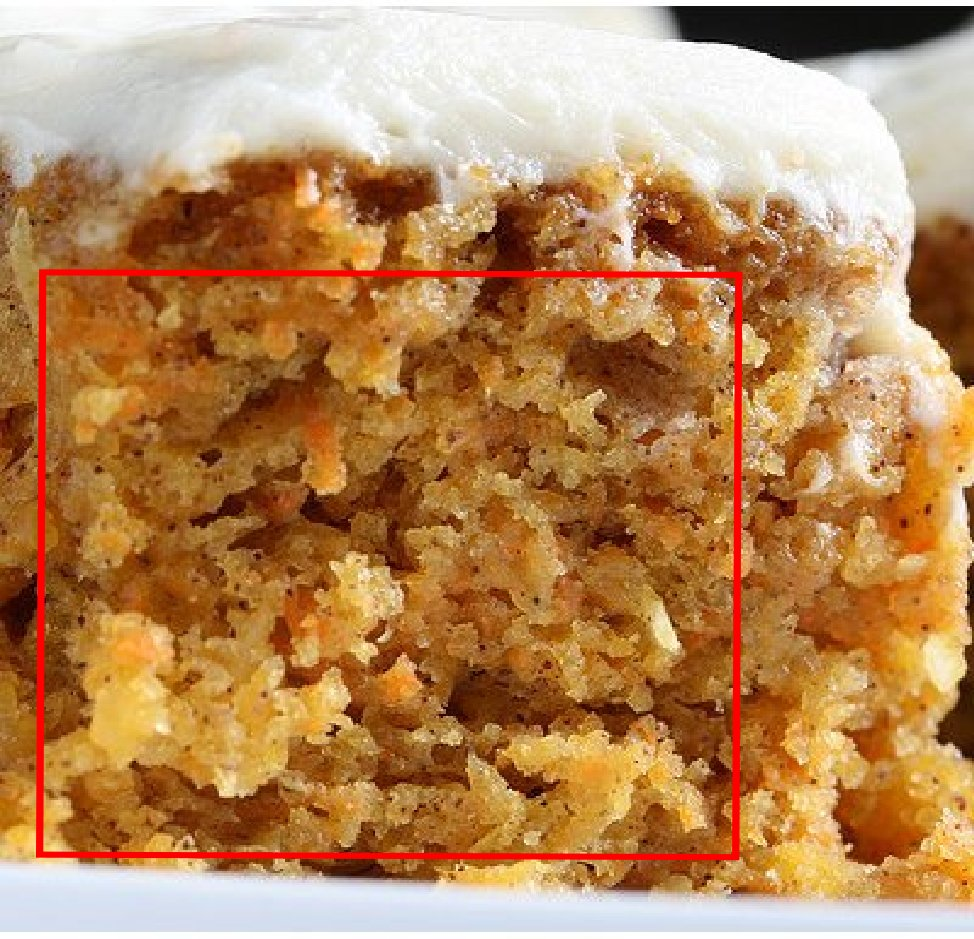
\includegraphics[width=0.24\linewidth, height=35mm]{./figs/2/2.jpg} & 
\hspace{-3mm}
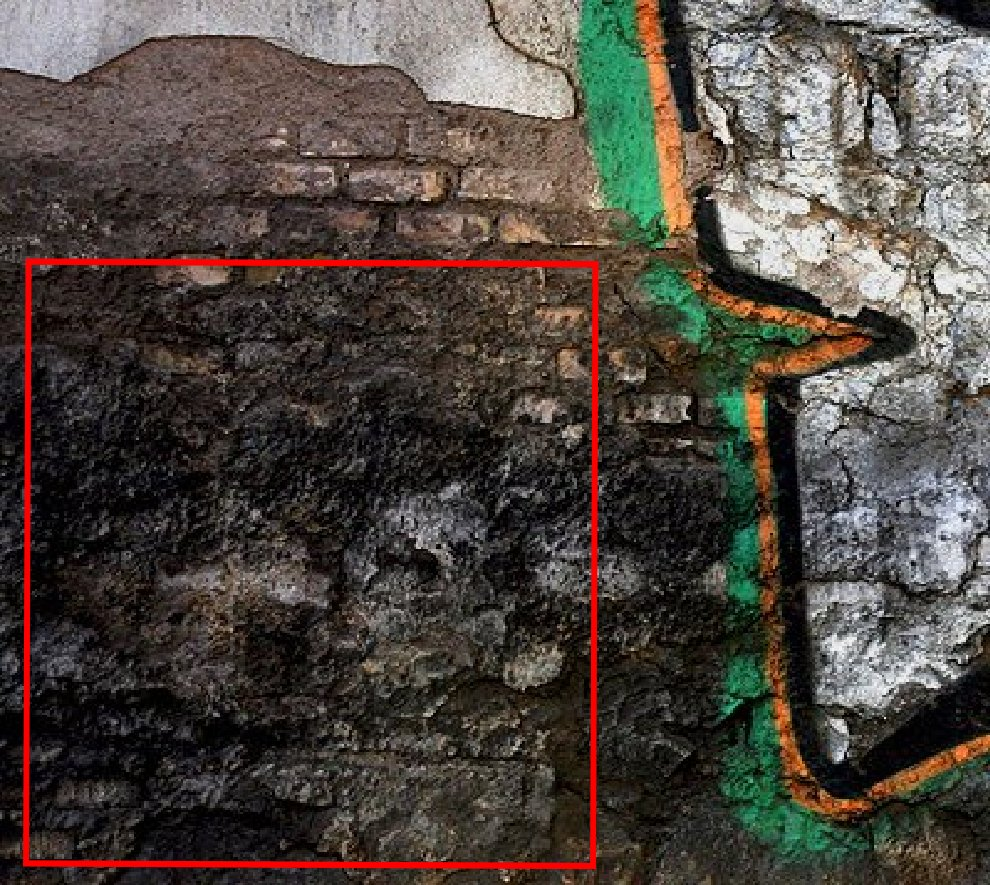
\includegraphics[width=0.24\linewidth, height=35mm]{./figs/2/3.jpg} & 
\hspace{-3mm}
\includegraphics[width=0.24\linewidth, height=35mm]{./figs/2/22_1.jpg} & 
\hspace{-3mm}
\includegraphics[width=0.24\linewidth, height=35mm]{./figs/2/22_3.jpg} \\
\scriptsize{\text{RS:\textcolor{red}{0.92} \hspace{1mm} IS:0.40}} & 
\scriptsize{\text{RS:\textcolor{red}{0.67}, \hspace{1mm} IS:0.50}}  &
\scriptsize{\text{RS:\textcolor{red}{0.63} \hspace{1mm} IS:0.42}} & 
\scriptsize{\text{RS:\textcolor{red}{0.74} \hspace{1mm} IS:0.43}} \\ 
\end{array}$
\caption{The most synthesizable region detected by our system. 
Synthesizability of detected regions (RS) and the whole images (IS) are shown. }
  \label{fig:roi}
\end{figure*}


\subsection{Texture characterization}
In this section, we show and compare the image synthesizability of
different texture categories.  The UIUC texture
dataset~\cite{UIUC:Texture}, which contains $25$ texture categories,
each with $40$ images. Fig.~\ref{} shows the synthesizability of all
categories (average of synthesizability of all texture examples in
each category). From the figure, we find that ... 

This characterization could be further analyzed in terms of different
texture materials, different illumination conditions, different scales
of textures, and so on. The characterization of textures of
Columbia-Utrecht Reflectance and Texture
Database~\cite{columbia:texture} and Open-Surface
dataset~\cite{open:surface} is planned as a future work. The former
one is about different illuminations, and the latter is for real-world
semantic textures.

\subsection{Texture recognition}
In this section, we evaluate the usefullness of synthesizability on
texture recognition. The UIUC texture dataset~\cite{UIUC:Texture} was again used. Linear SVMs was used
as the classifier, with $C=15$. We show the classification accuracy of
Unary LBP~\cite{lbp}, image synthesizability, and the concatenation of
both. The result is shown in Table~\ref{table:recognition}. From the table, ...

\begin{table}[tb] \footnotesize 
$\begin{array}{ccccc}
\begin{tabular}{|c||c||}
\hline 
\multicolumn{1}{|c||}{Feature} \\ \hline \hline
Accuracy \\  \hline
\end{tabular}

\begin{tabular}{|c|c|}
\hline
\multicolumn{1}{|c|}{LBP} \\ \hline \hline
63.8 (4.7)  \\ \hline
\end{tabular}

\begin{tabular}{|c|c|}
\hline 
\multicolumn{1}{|c|}{Syn} \\ \hline \hline
??   \\  \hline
\end{tabular}

\begin{tabular}{|c|c|}
\hline 
\multicolumn{1}{|c|}{LBP + Syn} \\ \hline \hline
??   \\  \hline
\end{tabular}
\end{array} $
\vspace{1mm}
\centering 
\caption{ Texture classification accuracy on Texture-25 dataset. 
} \label{table:recognition}
\end{table}
